\documentclass[12]{article}
\usepackage[utf8]{inputenc}
\usepackage{cite}
\usepackage{fullpage}
\usepackage{float}
\usepackage{subcaption}
\usepackage{graphicx}
\usepackage{amssymb}
\author{Xavier Martín Ballesteros and Adrià Cabeza Sant'Anna}
\title{Meat Quality Control \\ \large{Computer Vision, UPC}}

\begin{document}
\maketitle
  \vspace{1cm}
  %QUEDA MOLT CURT MAYBE HO PODRÍEM TREURE
%	\begin{abstract}
%Our goal is to detect the percentage of fat in chops using images. We discuss about the different binarization methods we have used, such as \textit{basic binarization}, \textit{p-tile thresholding}, \textit{optimal thresholding} and \textit{kapur method}. Finally, we have analysed our results and decided which method is the best one.
%\end{abstract}

\newpage
\tableofcontents
%podem posar un \newpage aquí si volem 
\section{Introduction}
%afegir coses tipus lo de la mascara i yasta
The objective of this assignment is to detect the percentage of fat in chops using images. To do it, we have used several different threshold techniques. Those methods consists in setting a constant value called \textit{threshold} ($T$) and separe the pixels depending its value ($ f(i,j)$):
\vspace{-0.6cm}
\begin{center}
$$ g(i,j)=1\ if\ f(i,j) \geq T$$ 
$$ g(i,j)=0\ if\ f(i,j) \leq T$$
\end{center}

In the following sections we will introduce different methods to find the threshold value and compared its results. 

\section{Binarization}
\subsection{Basic Binarization}
This is the first method we tried and also the fastest and easiest one. 

\noindent Our approach was to print the histogram of the picture and check where we could set the best value for the \textit{threshold} in order to separe the fat. The histograms that we got were bimodal so we coud set an acceptable value just by looking at it. We believe that this distribution of pixel values is formed because we are working with grayscale pictures of chops where we can appreciate clearly a lighter tone for the fat and darker tones for the rest.
\subsection{P-tile Method}
This method uses knowledge about the area size of the desired object. It assumes the desired part of the image are brighter that the background and occupy a fixed percentage of the picture area. The \textit{threshold} is defined as the grey level that mostly corresponds to mapping at least that fixed percentage into the object. 

\subsection{Otsu Method}
Otsu method is one of the most successful methods for image thresholding. It is very effective for images which are bimodal. However, it may not be accurate for non-bimodal images. In this method we search among all possible thresholds to find the one that minimizes the weighted within-class variance, which is the same than maximizing inter-class variance.

The probability of a pixel to have the gray level \textit{i} is
\vspace{-0.5cm}
\begin{center}
$$ p_i = \frac{n_i}{N}, \hspace{1cm} p_i \geqslant 0, \sum_{i = 0}^{L - 1} p_i = 1  $$
\end{center}
where L is the number of different gray levels of a given picture, $n_i$ is the number of pixels of gray level \textit{i} and \textit{N} is the total number of pixels. Then, the probability of being in class \textit{Background} or \textit{Foregound} is
\vspace{-0.5cm}
\begin{center}
$$ \omega_B = \sum_{i = 0}^{t} p_i \hspace{1cm} \omega_F = \sum_{i = t + 1}^{L} p_i $$
\end{center}
where \textit{t} is the threshold value. The mean values of the classes are
\vspace{-0.5cm}
\begin{center}
$$ \mu_B = \sum_{i = 0}^{t} \frac{i * p_i}{n_B} \hspace{1cm} \mu_F = \sum_{i = t + 1}^{L} \frac{i * p_i}{n_F} $$
\end{center}
and the class variances are given by
\vspace{-0.5cm}
\begin{center}
$$ \sigma_{B}^{2} = \sum_{i = 0}^{t} \frac{(i - \mu_B)^2 * n_i}{n_B} \hspace{1cm} \sigma_{F}^{2} = \sum_{i = t + 1}^{L} \frac{(i - \mu_F)^2 * n_i}{n_F} $$
\end{center}
Hence, the within-class variance is computed as
\vspace{-0.5cm}
\begin{center}
$$ \sigma_{W}^{2} = \omega_B * \sigma_{B}^{2} + \omega_F * \sigma_{F}^{2} $$
\end{center}
Nevertheless, we can transform this minimization problem into a maximization problem by computing the inter-class variance, which is faster to compute
\vspace{-0.5cm}
\begin{center}
% \sigma^{2} - \sigma_{W}^{2}
$$ \sigma_{I}^{2} = \omega_B * \omega_F * (\mu_F - \mu_B)^2 $$
\end{center}

\subsection{Optimal thresholding by Clustering Method}
Optimal thresholding methods select the threshold based on the minimization of a criterion function. Otsu, for example, tries to minimize the intra-class variance. This method tries to minimize the probability between the maxima of 2 distributions.

We used Ridler Calvard Method which segments the image into two clusters (\textit{Background} and \textit{Foreground}) using the initial theshold value. The algorithm starts assuming that the four corners are the only pixels in the \textit{Background} and the rest is the \textit{Foregound}. It also selects an initial estimate for the threshold \textit{$t_1$}. At each step we compute the mean gray-level of the two clusters
\vspace{-0.5cm}
\begin{center}
$$ \mu_{B}^{t_n} = \frac{\sum_{i = 0}^{t_n} i * p_i}{n_B} \hspace{1cm} \mu_{F}^{t_n} = \frac{\sum_{i = t_n + 1}^{L} i * p_i}{n_F} $$
\end{center}
Then, the new threshold is compute as
\vspace{-0.5cm}
\begin{center}
$$ t_{n + 1} = \frac{\mu_{B} + \mu_{F}}{2} $$
\end{center}
The algorithm repeats these steps until \textit{t} stabilizes, which means that $|t_n - t_{n + 1}| < \varepsilon $.

\subsection{Kapur, Sahoo and Wong Method}
Kapur, Sahoo and Wong Method is the method we have implemented from the entropic methods family. In this method we work with the gray level histogram to obtain the optimal threshold applying information theory.
The way it works is the following: two probability distributions are derived from the original gray level distribution of the image(i.e. object distribution and background distribution): 
\vspace{-0.5cm}
\begin{center}
$$\frac{p_0}{P_t},\frac{p_1}{P_t},...,\frac{p_t}{P_t}$$
\end{center} \begin{center}
and
$$\frac{p_{t+1}}{1-P_t},\frac{p_{t+2}}{1-P_t},...,\frac{p_{l-1}}{1-P_t}$$
\end{center}
\vspace{0.4cm}

where \textit{t} is the value of the threshold and $P_t = \sum_{i=0}^{t}{p_i}$. Then, we define

$$H_b(t) = - \sum_{i = 0}^{t} \frac{p_i}{P_t}log_e\left(\frac{p_i}{P_t}\right)$$
$$ H_b(t) = - \sum_{i = t+1}^{l-1} \frac{p_i}{1-p_i}log_e\left(\frac{p_i}{1-P_t}\right)$$

And finally the optimal threshold $t^{*}$ is defined as the grey level which maximizes $H_b(t)+H_w(t)$, that is, 
\vspace{-0.5cm}
\begin{center}
$$t^{*}=\ ArgMax\left(H_b(t) + H_w(t)\right)$$
\end{center}

%MIRAR 
In our implementation, in order to do all the loops using matricial operations we have inserted a tiny value ($1\times 10^{-3}$) as an intended error in our calculations because we wanted to avoid NaN because the division by 0 cases. 
\section{Results}
In the following section we will see the results of our methods being applied to the dataset given. A total of 14 chops images will be analysed to check how many fat do they have.  
Finally we will discuss which method was to best one and we will take our conclusions %maybe també hauríem de posar el valor del greix que hem trobat mirant l'histograma
\subsection{Table}
\begin{table}[H]
\centering
\begin{tabular}{|l|l|l|l|l|}
\hline	
Picture of the chop & \textbf{Otsu} & \textbf{Kapur} & \textbf{Optimal Thresholding} & \textbf{P-tile} \\  \hline
 F1011flb.bmp & 29.1682  & 31.3817 & 29.2252  & 39.5698  \\ \hline
  F1019flb.bmp & 33.2429 & 36.2029 & FALLA A SACO & 39.5983 \\  \hline
  F1031flb.bmp & 38.1320 & 44.5639 & 38.4935 & 39.2967  \\ \hline
  F1051flb.bmp & 33.8235 & 36.8900 & 35.6833 & 39.5664\\ \hline
F1053flb.bmp & 35.6418 & FALLA A SACO & 35.6833 & 37.8899\\ \hline
F1059flb.bmp & 28.4953 & FALLA & FALLA & FALLA \\ \hline
F1064flb.bmp & 26.4423 & 26.0063 & 27.1537 & FALLA A SACO\\ \hline
F1079f1b.bmp & 31.2544 & FALLA &  FALLA & FALLA \\ \hline
F1083f1b.bmp & 27.5718 & FALLA & 27.7740  & FALLA \\ \hline
F1096f1b.bmp & 28.8945 & FALLA & FALLA & FALLA \\ \hline
F1097flb.bmp & 29.2960 & FALLA & FALLA & FALLA \\ \hline
F1101flb.bmp & 33.2675 & FALLA & 34.7553 & FALLA \\ \hline
F1102f1b.bmp & 27.6687 &FALLA &FALLA	 & FALLA \\ \hline
F1103f1b.bmp  & 34.0777 & FALLA & 37.7081 & 39.6781\\ \hline
\end{tabular}
\caption{Results obtained using different methods of binarization}
\label{Results}
\end{table}


Even though we already know that \textit{P-tile} does not make sense for this assignment we have implemented it because we wanted to expand our knowledge about different algorithms related to find the optimal threshold automatically. 

After experimenting with several different values for the percentage we have set it to 70\% which gave us the best results. 

\subsection{Images}

\begin{figure}[H]
\begin{subfigure}{.5\textwidth}
  \centering
  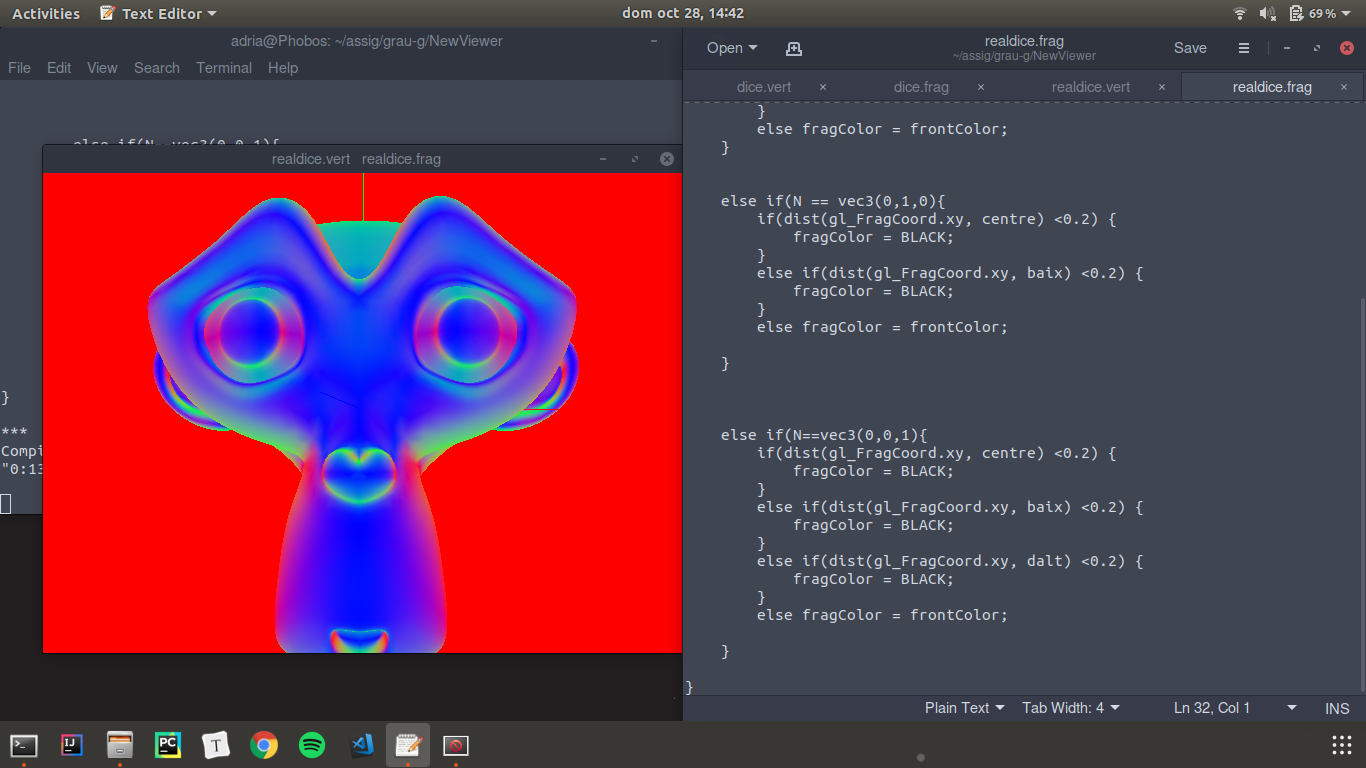
\includegraphics[width=.8\linewidth]{a.png}
  \caption{1a}
  \label{fig:sfig1}
\end{subfigure}%
\begin{subfigure}{.5\textwidth}
  \centering
  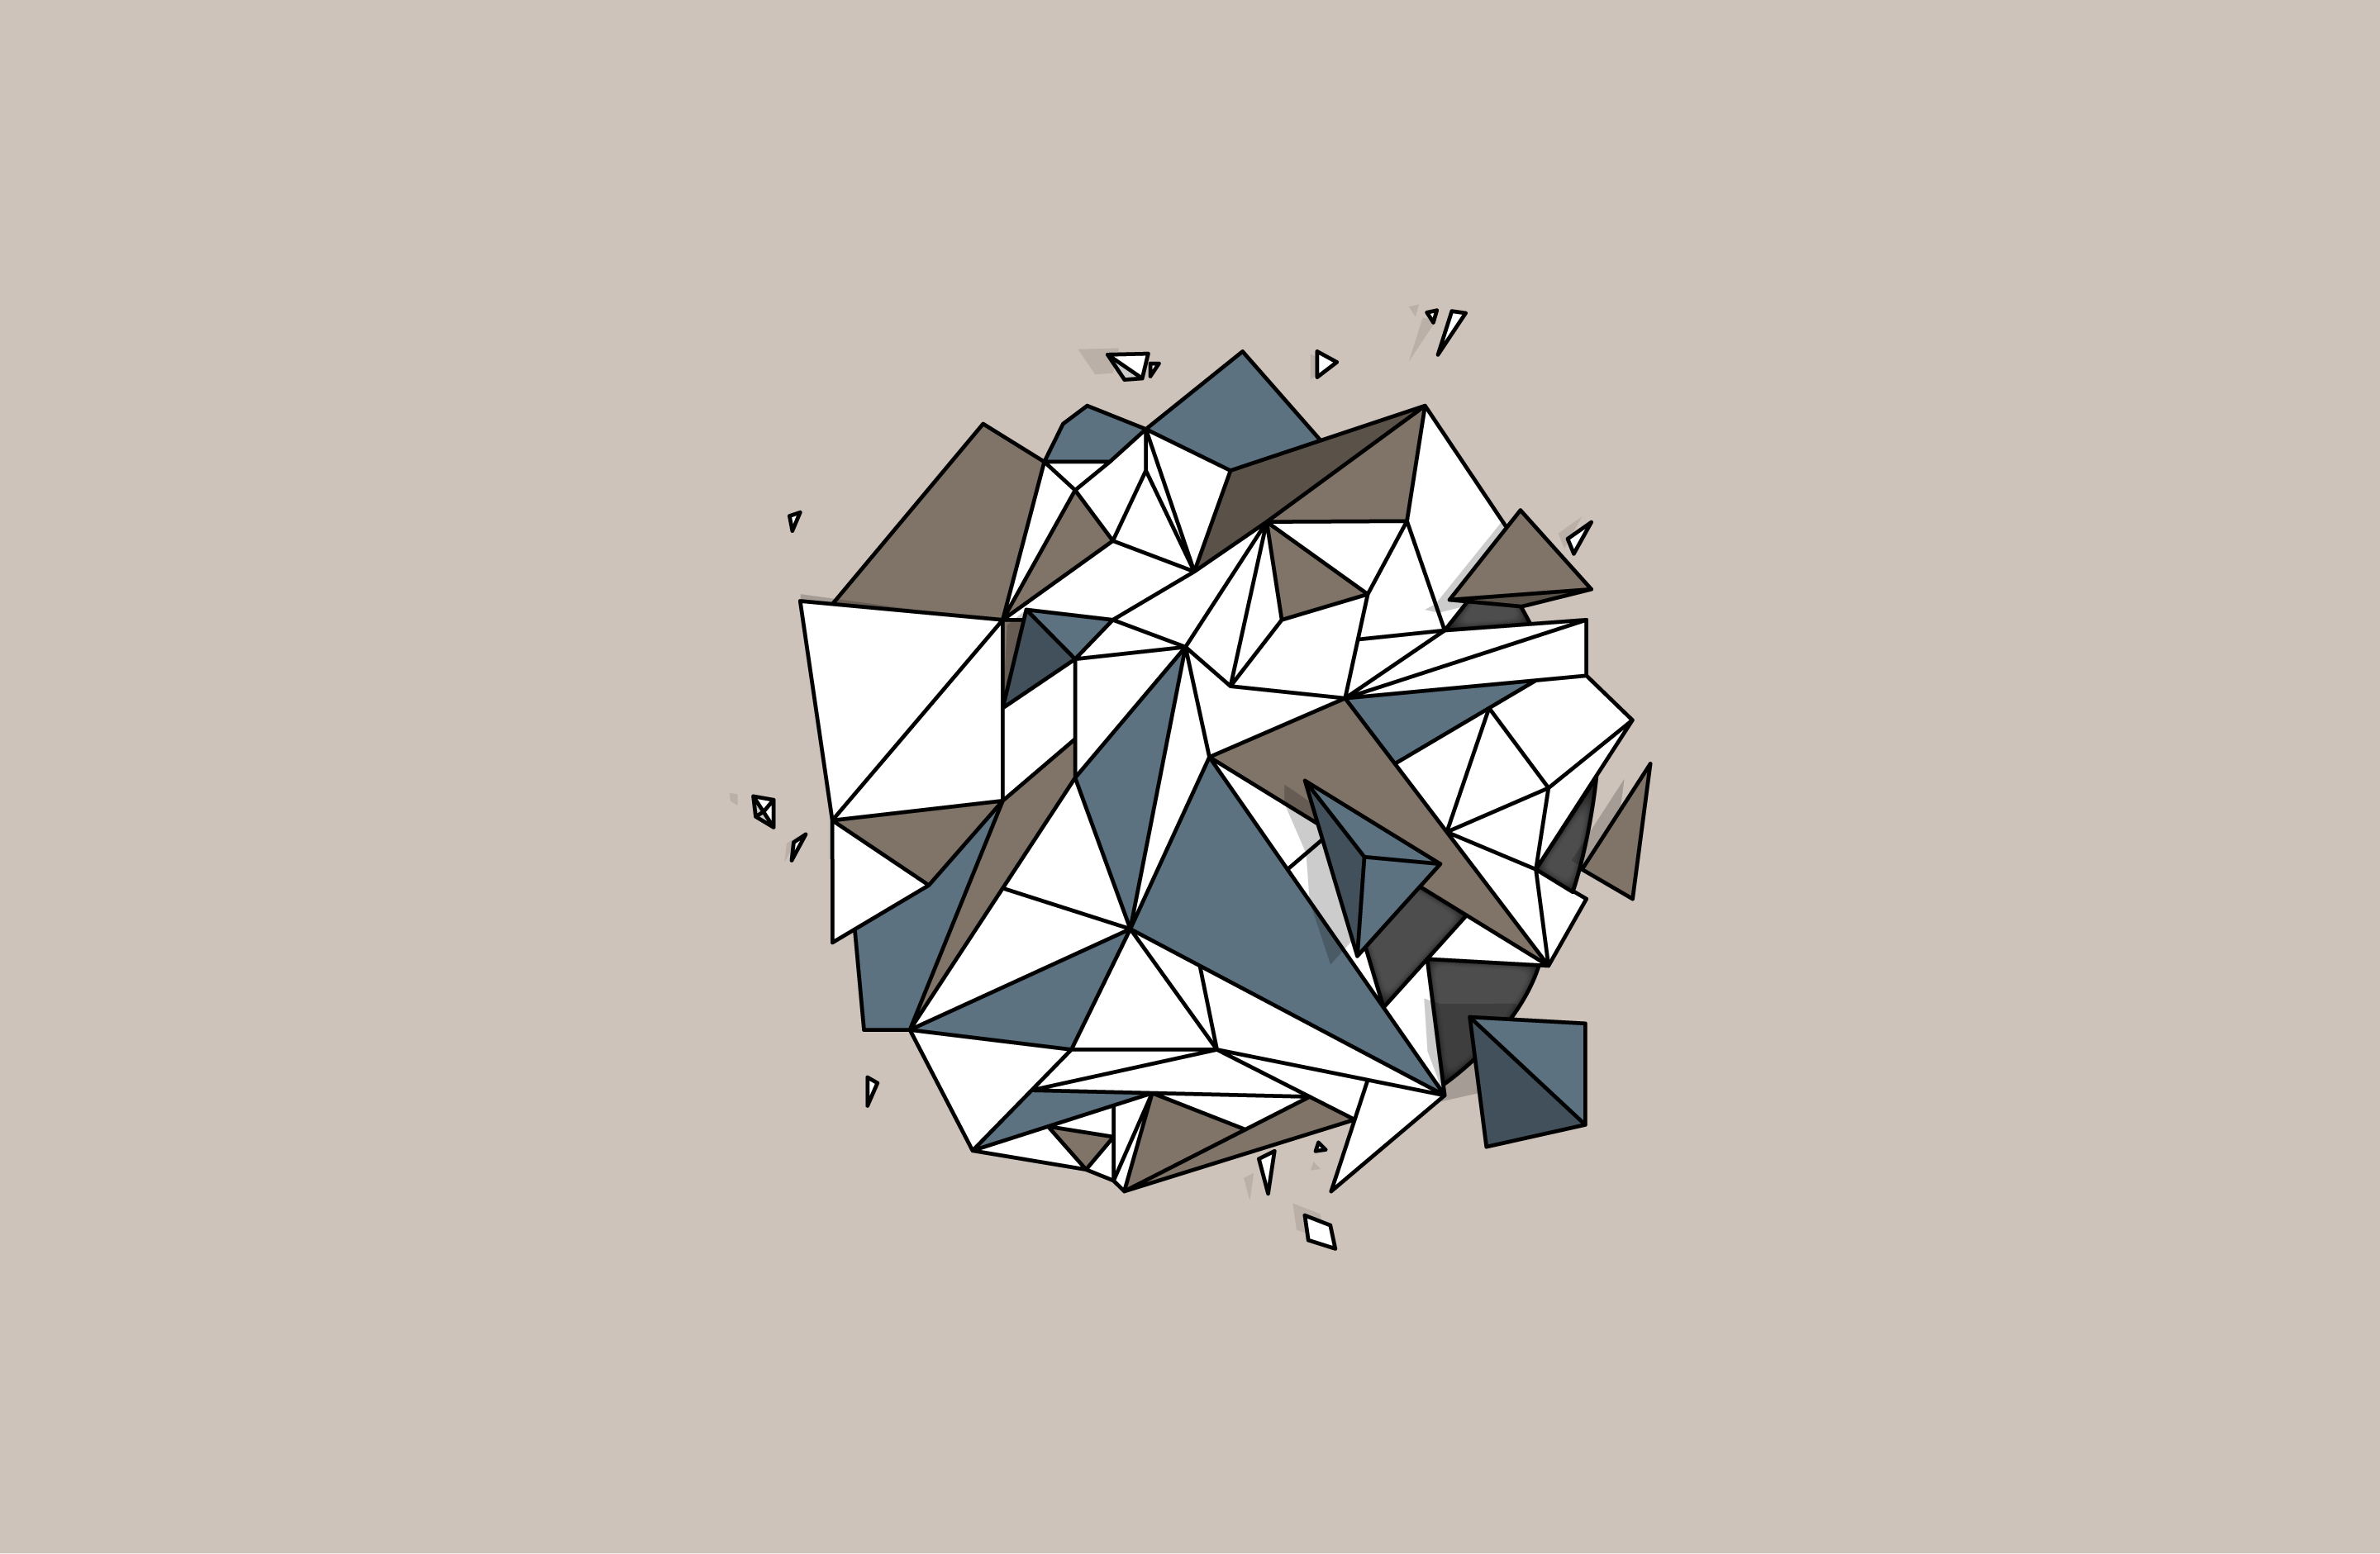
\includegraphics[width=.8\linewidth]{polymagnet.png}
  \caption{1b}
  \label{fig:sfig2}
\end{subfigure}
\caption{plots of....}
\label{fig:fig}
\end{figure}



\begin{thebibliography}{100}

\bibitem{A Comparison of Thresholding Methods - NTNU}
C. Henden (2004). \textit{ Exercise in Computer Vision. A Comparison of Thresholding Methods.} [online] NTNU. Available at: http://www.pvv.org/~perchrh/papers/datasyn/paper2/report.pdf [Accessed 14 Mar. 2019].


\bibitem{Analysis of image Thresholding Methods for application to augmented reality enviornments}
D. Martín Carabias (2012). \textit{Analysis of image Thresholding Methods for application to augmented reality enviornments.} [online] UCM. Available at: https://eprints.ucm.es/16932/1/Tesis\_Master\_Daniel\_Martin\_Carabias.pdf [Accessed 14 Mar. 2019].


\bibitem{A survey of Thresholding Techniques}
P. K. Sahoo, S. Soltani, K.C. Wong and Y.C. Chen (1988). \textit{A survey of Thresholding Techniques}. University of Waterloo, Waterloo, Canada  [Accessed 16 Mar. 2019].

\bibitem{}N. Otsu, \textit{A Threshold Selection Method from Gray-Level Histograms}, in IEEE Transactions on Systems, Man, and Cybernetics, vol. 9, no. 1, pp. 62-66, Jan. 1979.
[online] Available at http://ieeexplore.ieee.org/stamp/stamp.jsp?tp=\&arnumber=4310076\&is
number=4310064 [Acessed 17 Mar. 2019].

\bibitem{}Dr. Andrew Greensted (2010), \textit{Otsu Thresholding}. [online]. Available at http://www.labbookpages.co.uk/software/imgProc/otsuThreshold.html [Accessed 17 Mar. 2019].

\bibitem{}Senthilkumaran,  N.  \&  Sivapriya,  M.  (2017),  \textit{Riddler's  Thresholding Algorithm  for  DNA  Image  Using  ISODATA  Modified  Algorithm} Journal  of Information Technology, Vol.3, No.2, pp.41-48. [online] Available at: http://www.ijitjournal.org/volume-3/issue-2/IJIT-V3I2P9.pdf [Accessed 17 Mar. 2019].

%TODO ficar els apunts del profe a bibliografia 
\end{thebibliography}

91 160
112 200
100 190
105 200
78 158
57 168
75 160
69 186
66 165
54 160
63 165
66 170
67 170
54 153


\end{document}